\section{Modelos de classifica\c{c}\~{a}o e sensores analisados}

\begin{figure}[tbh!]
	\centering
	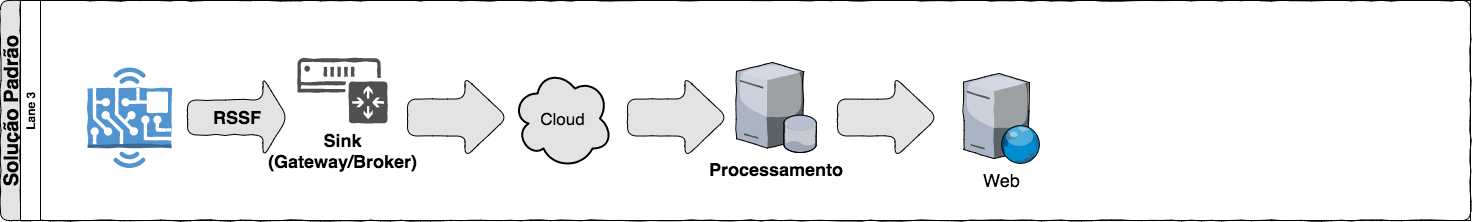
\includegraphics[width=1.0\textwidth]{../images/padrao_rede}
	\caption{Arquitetura RSSF padr�o}
	\label{fig:rssfpadrao}
\end{figure}

Em \cite{Ueyama002840382} e \cite{Furquim002744726}, uma estrutura de sensores do tipo b\'{o}ia foi criada para coleta e an�lise do n�vel da �gua e sua polui��o em rios.

\begin{figure}[tbh!]
	\centering
	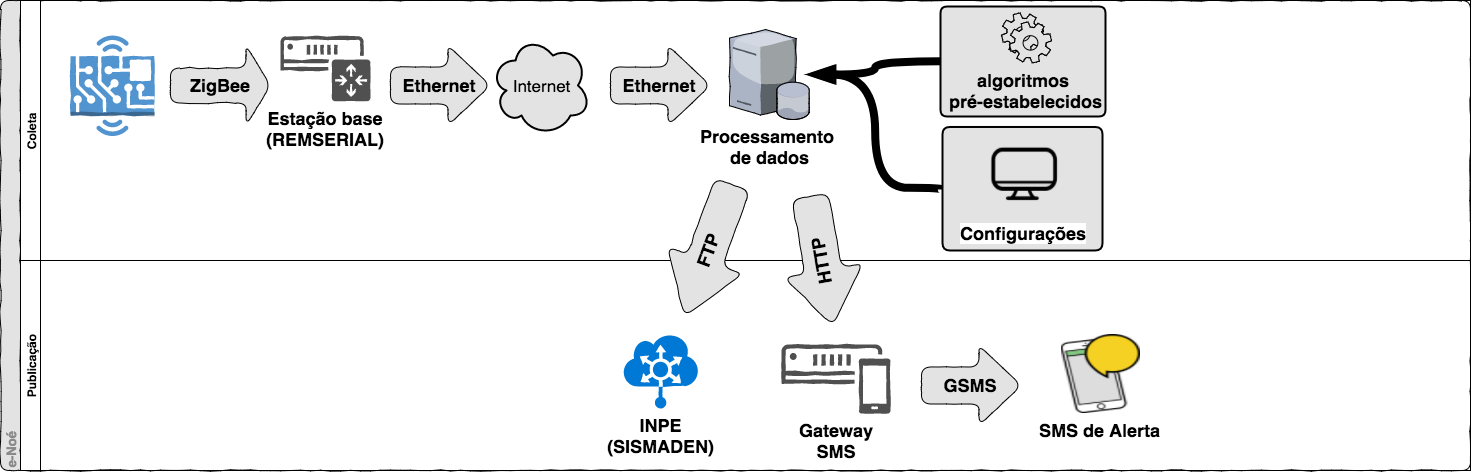
\includegraphics[width=1.0\textwidth]{../images/enoe_rede}
	\caption{Projeto e-No�}
	\label{fig:enoe}
\end{figure}

De acordo com o trabalho realizado em \cite{Chen2014}, podemos analisar, classificar e quantificar os insetos encontrados em uma determinada regi�o utilizando sensores ac�sticos, de forma a utilizar os resultados encontrados para aplica��o de uma quantidade determinada de defencivos, controlando o efeito de sua aplica��o em tempo real.

Utilizando m�tricas encontradas em \cite{}

Um outro problema que eu vi potencial, seria uma solu\c{c}\~{a}o de custo reduzido para controle automatizado de uso de recursos em m�todos alternativos de agricultura. 
Na pr�tica seria usar RSSF, sensores, atuadores e um sistemas distribu�do para automatizar processos como o de gotejamento localizado como descrito nas imagens abaixo, baseado em informa\c{c}\~{o}es retiradas da bdpa (base de pesquisas agropecu�ria) da embrapa.

\begin{figure}[!htb]
	\centering
	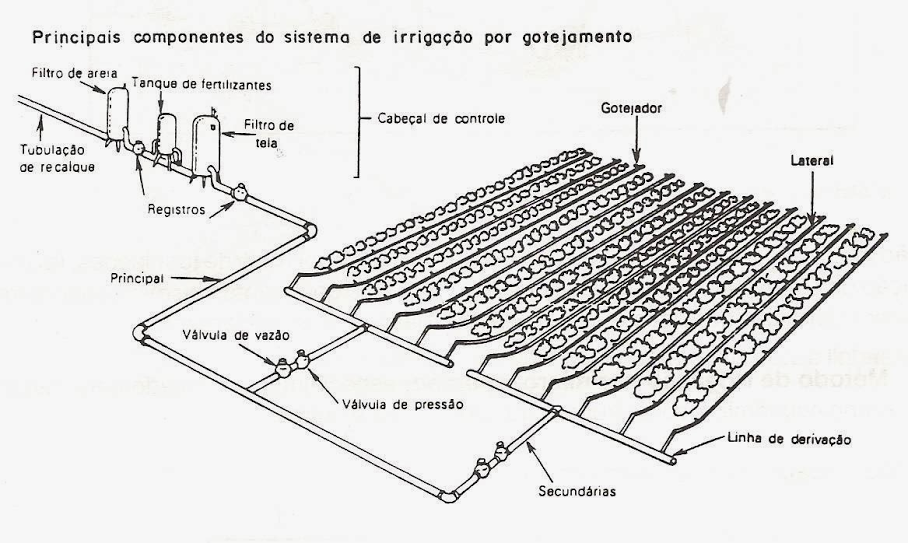
\includegraphics[width=1.0\textwidth]{../images/irrigacao.png}
	\caption{Principais componentes de um sistema de irriga\c{c}\~{a}o}
	\label{fig:irrigacao}
\end{figure}

\begin{figure}[!htb]
	\centering
	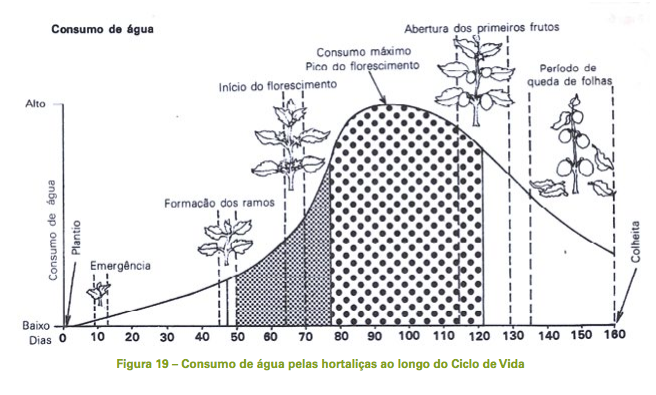
\includegraphics[width=1.0\textwidth]{../images/consumo_de_agua.png}
	\caption{Consumo de �gua}
	\label{fig:consumoagua}
\end{figure}



\begin{table}[]
	\centering
	\caption{Consumo de \'{a}gua para diferentes hortali\c{c}as durante o seu desenvolvimento}
	\label{table:consumo1}
	\begin{tabular}{lc}
		\hline
		Cultura	& Consumo de �gua/min\(mm\)	\\ 
		\hline
		Batata				& 500 a 800 \\
		Batata-doce			& 400 a 675 \\
		Beterraba			& 100 a 1500 \\
		Cebola				& 350 a 600 \\
		Feij�o-de-vagem		& 300 a 500 \\
		Milho-verde			& 400 a 700 \\
		Tomate				& 300 a 600 \\
		Outras hortali�as	& 250 a 500 \\ \hline
	\end{tabular}
\end{table}

\begin{table}[]
	\centering
	\caption{Per\'{i}odos cr\'{i}ticos de defici\^{e}ncia de \'{a}gua para v\'{a}rias hortali\c{c}as}
	\label{table:periodocritico}
	\begin{tabular}{ll}
		\hline
		Cultura	& Consumo de �gua/min\(mm\)\\ 
		\hline
		Alface				& 500 a 800 \\
		Batata-doce			& 400 a 675 \\
		Beterraba			& 100 a 1500 \\
		Cebola				& 350 a 600 \\
		Feij�o-de-vagem		& 300 a 500 \\
		Milho-verde			& 400 a 700 \\
		Tomate				& 300 a 600 \\
		Outras hortali�as	& 250 a 500 \\
		\hline
	\end{tabular}
\end{table}

\begin{table}[]
	\centering
	\caption{Tempo (em horas) necess�rio para irrigar diariamente as culturas do milho, melancia, banana e mam\~{a}o, em fun\c{c}\~{a}o da idade da planta (DAP) e do m\^{e}s do ano.Para os sistemas com aspers\~{a}o convencional, o intervalo entre irriga\c{c}\~{o}es � de 4 dias.}
	\label{table:consumo2}
	\begin{tabular}{lllllllllllll}
		\hline
		\multicolumn{13}{l}{Milho com uso de microdifusor \(42 l/h\)} \\
		\hline
		DAP	& Jan. & Fev. & Mar. & Abr. & Mai. & Jun. & Jul. & Ago. & Set. & Out. & Nov. & Dez. \\
		At� 25& 0,4& 0,4& 0,4& 0,4& 0,3& 0,3& 0,3& 0,3& 0,5& 0,5& 0,5& 0,4 \\
		26 - 55& 0,7& 0,7& 0,6& 0,6& 0,5& 0,5& 0,5& 0,5& 0,7& 0,8& 0,8& 0,7 \\
		56 - 95& 0,6& 0,6& 0,6& 0,6& 0,5& 0,4& 0,4& 0,5& 0,7& 0,7& 0,7& 0,6 \\
		\hline
		\multicolumn{13}{l}{Melancia com uso de microdifusor \(42 l/h\)} \\ 
		\hline
		DAP & Jan. & Fev. & Mar. & Abr. & Mai. & Jun. & Jul. & Ago. & Set. & Out. & Nov. & Dez. \\			
		At� 25& 0,2& 0,2& 0,2& 0,2& 0,2& 0,2& 0,1& 0,2& 0,2& 0,2& 0,2& 0,2 \\
		25-50& 0,7& 0,7& 0,6& 0,6& 0,5& 0,5& 0,4& 0,5& 0,7& 0,7& 0,7& 0,7 \\
		50-70& 0,4& 0,4& 0,3& 0,3& 0,3& 0,3& 0,2& 0,3& 0,4& 0,4& 0,4& 0,4 \\
		\hline
		\multicolumn{13}{l}{Banana com uso de microdifusor \(42 l/h\)} \\
		\hline
		DAP & Jan. & Fev. & Mar. & Abr. & Mai. & Jun. & Jul. & Ago. & Set. & Out. & Nov. & Dez. \\			
		At� 30& 0,3& 0,3& 0,3& 0,3& 0,2& 0,2& 0,2& 0,2& 0,3& 0,3& 0,3& 0,3 \\
		31 - 210& 0,7& 0,7& 0,6& 0,6& 0,5& 0,5& 0,5& 0,5& 0,7& 0,8& 0,8& 0,7 \\
		211 - 365& 0,6& 0,6& 0,6& 0,6& 0,5& 0,4& 0,4& 0,5& 0,7& 0,7& 0,7& 0,6 \\
		\hline
		\multicolumn{13}{l}{Mam\~{a}o com uso de microdifusor \(42 l/h\)} \\
		\hline
		DAP & Jan. & Fev. & Mar. & Abr. & Mai. & Jun. & Jul. & Ago. & Set. & Out. & Nov. & Dez. \\	
		At� 107& 0,4& 0,4& 0,4& 0,4& 0,3& 0,3& 0,3& 0,3& 0,4& 0,4& 0,4& 0,4 \\
		108 - 260& 0,7& 0,7& 0,7& 0,6& 0,6& 0,5& 0,5& 0,6& 0,8& 0,8& 0,8& 0,7 \\
		261 - 380& 0,7& 0,7& 0,7& 0,7& 0,6& 0,5& 0,5& 0,6& 0,8& 0,8& 0,8& 0,8 \\
		\hline
	\end{tabular}
\end{table}